\documentclass[conference]{IEEEtran}
\IEEEoverridecommandlockouts

% EDITORIAL POLICY -- preserve this comment in all future revisions.
% This paper presents a general, runtime-neutral agent harness design.
% Do not mention Pi Agent or its implementation identity in rendered text,
% figure labels/captions, screenshots, acknowledgments, or references.
% Use "coding agent", "agent engine", "agent adapter", and "run supervisor".
% Do not reintroduce runtime-specific package URLs, class names, or executable
% names when consulting the implementation. Describe the integration contract
% generically, while retaining the actual measured results and limitations.

\usepackage{cite}
\usepackage{amsmath,amssymb,amsfonts}
\usepackage{algorithm}
\usepackage{algpseudocode}
\usepackage{graphicx}
\usepackage{textcomp}
\usepackage{xcolor}
\usepackage{booktabs}
\usepackage{multirow}
\usepackage{tikz}
\usetikzlibrary{positioning,arrows.meta,fit,calc,patterns}
\usepackage[hidelinks]{hyperref}

\newcommand{\code}[1]{\texttt{\small #1}}

\begin{document}

\title{A Harness for Automating Agent-Driven\\Memory Repair Evaluation}

\author{\IEEEauthorblockN{Author Name}
\IEEEauthorblockA{\textit{Affiliation} \\
City, Country \\
email@example.com}}

\maketitle

\begin{abstract}
Evaluating a memory redundancy architecture on wafer data is usually a
manual workflow: an engineer hand-writes architecture-specific repair code,
compiles it, runs it wafer by wafer, and tallies yield figures into
comparisons. Each new configuration repeats this loop. This report
describes a harness, the core of the self-hosted Pixel Chat workspace,
that automates the whole loop instead of hand-making each evaluation. A
user selects architectures and wafers. The harness then queues one job per
pair, starts a supervised LLM agent to write a narrow C++ model for each
architecture, compiles and runs it under resource limits, and refreshes
saved conclusions as jobs finish, without further human steps. The
harness's purpose is automation, not proof of correctness: its protocol,
invariant and input-hash checks exist so that runs can proceed unattended
and stay traceable, and they do not verify that the generated repair code
is optimal or correct. Under explicit, stated planning assumptions, the
harness reduces the estimated engineering effort per configuration by about
an order of magnitude, so the same team can evaluate many more design
candidates; these are scenario estimates, not measured human productivity.
We describe the process supervision, run and job state machines, event
log, and recovery rules, and report a real batch that completed in minutes,
with agent code generation taking most of the time and compilation and
solving only a small fraction.
\end{abstract}

\begin{IEEEkeywords}
LLM agents, agent harness, evaluation automation, process supervision, memory repair, redundancy analysis
\end{IEEEkeywords}

%======================================================================
\section{Introduction}
%======================================================================

Memory arrays carry spare rows and columns so that failing cells can be
replaced at wafer test. Choosing the spare budget is an early architectural
decision, and evaluating a candidate means encoding it as a repair model,
running the model on wafer fail maps, and aggregating yields. Redundancy
analysis is NP-complete in its classical form~\cite{kuo1987}, and every new
architecture variant needs new modelling code.
That implementation effort also limits how many spare-budget candidates an
engineering team can explore. A useful harness should therefore reduce the
human work per configuration, while preserving the evidence needed to
review the generated model and its results.

Coding agents that interleave reasoning and tool use~\cite{yao2023} can now
complete repository-level programming tasks~\cite{jimenez2024}, so the
modelling step can be delegated. Delegation alone does not remove the
engineer from the loop, however. An agent may hang, write files outside its
area, or leave background processes; a user may cancel midway, the service
may restart, and results must still be matched to their inputs. Without
something handling these cases, an engineer would still have to start,
watch, and clean up every run by hand. What makes the workflow automatic is
the \emph{harness}: the code around the agent that decides what it
receives, what it may do, what is accepted from it, and how each step is
recorded. Its checks keep unattended runs bounded and traceable; they are
not a proof that the generated repair code is correct, which remains a
matter for review.

This report describes that harness in Pixel Chat. Our contributions are:
\begin{itemize}
\item \textbf{A supervised agent run harness}
(Section~\ref{sec:runs}): per-run process groups with descendant tracking,
a strict line-delimited RPC protocol, a scoped context and toolset, an
append-only event log streamed over resumable Server-Sent
Events~\cite{sse}, and reconciliation from the agent's own session log.
\item \textbf{An automatic Solver pipeline} (Section~\ref{sec:pipeline}): a
durable queue that turns an architecture $\times$ wafer selection into jobs,
shares one code-generation run per architecture, and accepts a result only
after protocol, invariant, and input-integrity checks.
\item \textbf{A narrow agent output contract} (Section~\ref{sec:contract}):
the agent writes only an additive Pool/Action model behind a fixed,
validating solver core, and must declare constraints it cannot express.
\item \textbf{An operational study} (Section~\ref{sec:operation}) of a real
batch, including timings, agent tool traces, screenshots of the system in
use, an audit of the results, and an explicit engineering-effort estimate:
55.76 engineer-hours released across three configurations under the stated
productivity and review-budget assumptions.
\end{itemize}

%======================================================================
\section{Task Model}
\label{sec:problem}
%======================================================================

Data are organized as Product $\rightarrow$ Wafer $\rightarrow$ Chip
$\rightarrow$ Region. A region (a bank) is the independent repair unit. For
the reference product DEJOA, a region has $32768$ rows by $2048$ columns and
a chip has 16 regions. Each region has one pool of $R$ spare rows shared by
all of its row \emph{segments}; a row action covers every fail on one row.
Inside each segment, columns are split into $G$ CCR subgroups by
$c \bmod G$, and subgroup $k$ owns $C_k$ spare columns that serve only that
segment. Segments come from an inherited section/subsection row mapping, so
they need not be equal in length.

For one region with fail set $F$, candidate actions $A$ (only rows and local
columns that contain fails) each cover $F_a\subseteq F$ and use $w_{a,p}$
units of pool $p$ with capacity $K_p$. The region is repairable if some
$x\in\{0,1\}^{|A|}$ satisfies
\begin{equation}
\sum_{a: f\in F_a} x_a \ge 1\ \ \forall f\in F,\qquad
\sum_a w_{a,p}x_a \le K_p\ \ \forall p. \label{eq:model}
\end{equation}
\emph{Region yield} is the fraction of regions that are fail-free or
repaired. \emph{Chip yield} is the fraction of chips whose regions all pass.
\emph{Chip yield gain} is chip yield minus the fail-free chip fraction. A
region the heuristic cannot repair is \emph{unresolved}, not infeasible.

Wafers are stored in a sparse binary format (\code{PXLWAF1}): a 44-byte
header with a CRC-32, then delta-encoded LEB128 region and cell indexes,
which takes 2.5--2.8 bytes per fail on our wafers. Synthetic wafers come from
a seeded spatial Gamma--Poisson generator in the spirit of clustered yield
models~\cite{stapper1986,bae2007} and wafer-pattern studies~\cite{wu2015}.
Its parameters are \emph{not} fitted to measured data.

%======================================================================
\section{Harness Overview}
\label{sec:overview}
%======================================================================

\begin{figure}[t]
\centering
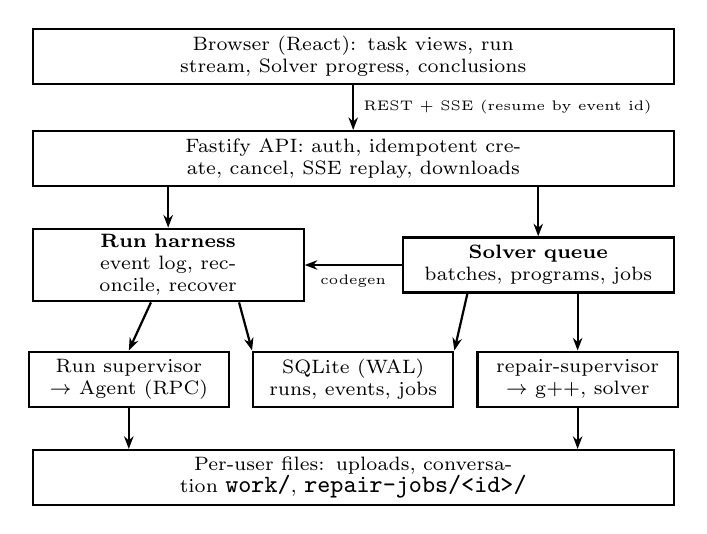
\begin{tikzpicture}[
  font=\scriptsize,
  box/.style={draw, thick, align=center, inner sep=2pt, minimum height=7mm},
  arr/.style={-{Stealth[length=1.6mm]}, thick}]
\node[box, text width=80mm] (ui) at (0,0) {Browser (React): task views, run stream, Solver progress, conclusions};
\node[box, text width=80mm] (api) at (0,-1.3) {Fastify API: auth, idempotent create, cancel, SSE replay, downloads};
\node[box, text width=33mm] (runs) at (-2.35,-2.65) {\textbf{Run harness}\\event log, reconcile, recover};
\node[box, text width=33mm] (rep) at (2.35,-2.65) {\textbf{Solver queue}\\batches, programs, jobs};
\node[box, text width=24mm] (agent) at (-2.85,-4.1) {Run supervisor\\$\rightarrow$ Agent (RPC)};
\node[box, text width=24mm] (db) at (0,-4.1) {SQLite (WAL)\\runs, events, jobs};
\node[box, text width=24mm] (rs) at (2.85,-4.1) {repair-supervisor\\$\rightarrow$ g++, solver};
\node[box, text width=80mm] (fs) at (0,-5.35) {Per-user files: uploads, conversation \code{work/}, \code{repair-jobs/<id>/}};
\draw[arr] (ui) -- node[right, font=\tiny]{REST + SSE (resume by event id)} (api);
\draw[arr] (api.south -| runs) -- (runs);
\draw[arr] (api.south -| rep) -- (rep);
\draw[arr] (rep) -- node[below, font=\tiny]{codegen} (runs);
\draw[arr] (runs) -- (agent.north -| runs.south -| agent);
\draw[arr] (runs.south) ++(0.9,0) -- (db.north west);
\draw[arr] (rep.south) ++(-0.9,0) -- (db.north east);
\draw[arr] (rep.south -| rs) -- (rs);
\draw[arr] (agent) -- (fs.north -| agent);
\draw[arr] (rs) -- (fs.north -| rs);
\end{tikzpicture}
\caption{Harness components. A Solver job uses the run harness for code
generation, then its own supervisor for compilation and solving.}
\label{fig:arch}
\end{figure}

The harness is part of one Node.js service with a SQLite database in
write-ahead-logging mode (Fig.~\ref{fig:arch}). We designed it around five
goals:
\begin{itemize}
\item[G1] \textbf{Bounded.} Every agent run, compile and solve has a
deadline, an output quota, and a process group that can be killed as a
whole.
\item[G2] \textbf{Checked.} Nothing the agent or solver produces is trusted
without validation: the model before solving, the protocol during it, and
the summary and inputs afterwards.
\item[G3] \textbf{Recoverable.} Retries are idempotent, cancellation always
terminates, and a restart never replays a paid agent call or presents a
partial result as complete.
\item[G4] \textbf{Observable.} Every agent event is persisted before it is
shown, and every job leaves a manifest and logs that can be downloaded.
\item[G5] \textbf{Comparable.} Each result carries the hashes of its wafer,
generated code and solver core, plus the architecture fingerprint.
\end{itemize}
These limits contain mistakes; they are \emph{not} a security sandbox. The
service is intended for internal teams on a trusted host.

%======================================================================
\section{Agent Run Harness}
\label{sec:runs}
%======================================================================

The agent-facing boundary is a runtime adapter for prompt submission,
typed event delivery, tool requests, cancellation and session recovery.
The harness owns the queue, process supervision, acceptance checks and
archived evidence; the agent engine supplies the architecture-specific
model. This separation expresses the design in terms of an integration
contract rather than a particular coding-agent implementation.

\subsection{Process tree and channels}

\begin{figure}[t]
\centering
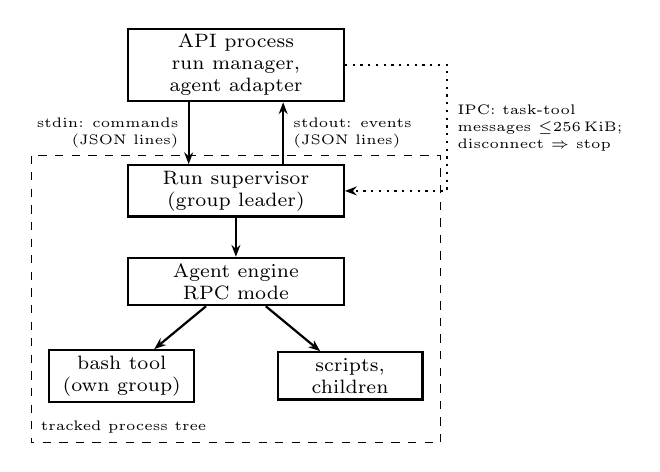
\begin{tikzpicture}[
  font=\scriptsize,
  p/.style={draw, thick, align=center, inner sep=2pt, minimum height=6mm, text width=26mm},
  arr/.style={-{Stealth[length=1.5mm]}, thick}]
\node[p] (be) at (0,0) {API process\\run manager, agent adapter};
\node[p] (sup) at (0,-1.6) {Run supervisor\\(group leader)};
\node[p] (agent) at (0,-2.75) {Agent engine\\RPC mode};
\node[p, text width=17mm] (t1) at (-1.45,-3.95) {bash tool\\(own group)};
\node[p, text width=17mm] (t2) at (1.45,-3.95) {scripts,\\children};
\draw[dashed] (-2.6,-1.15) rectangle (2.6,-4.8);
\node[anchor=south west, font=\tiny] at (-2.6,-4.8) {tracked process tree};
\draw[arr] ($(be.south)+(-0.6,0)$) -- node[left, font=\tiny, align=right]{stdin: commands\\(JSON lines)} ($(sup.north)+(-0.6,0)$);
\draw[arr] ($(sup.north)+(0.6,0)$) -- node[right, font=\tiny, align=left]{stdout: events\\(JSON lines)} ($(be.south)+(0.6,0)$);
\draw[arr, dotted] (be.east) -- ++(1.3,0) |- node[pos=0.25, right, font=\tiny, align=left]{IPC: task-tool\\messages $\le$256\,KiB;\\disconnect $\Rightarrow$ stop} (sup.east);
\draw[arr] (sup) -- (agent);
\draw[arr] (agent) -- (t1);
\draw[arr] (agent) -- (t2);
\end{tikzpicture}
\caption{Process tree of one agent run. Standard I/O passes through the
supervisor to the agent engine; the IPC channel carries task-tool traffic and signals
backend death.}
\label{fig:proc}
\end{figure}

Each run starts a small supervisor as a detached process group with an IPC
channel, and the supervisor starts the coding agent through the runtime
adapter in RPC mode
(Fig.~\ref{fig:proc}). Three mechanisms keep the run bounded:
\begin{itemize}
\item \textbf{Descendant tracking.} On Linux the supervisor snapshots its
process tree from \code{/proc} every 250\,ms and records each descendant's
start time. Agent shell tools may start their own process groups, so a plain group
kill would miss them. On stop, the supervisor signals each recorded process
whose start time still matches, which avoids killing a recycled PID. It sends
\code{SIGTERM}, then \code{SIGKILL} after 1.5\,s.
\item \textbf{Parent liveness.} If the API process dies, the IPC channel
closes and the supervisor stops the whole tree, so orphaned agents cannot
keep writing.
\item \textbf{Deadlines.} The run has a wall-clock limit (3600\,s by
default), each RPC command has a 30\,s response timeout, and stop escalates
from \code{SIGTERM} to \code{SIGKILL} on the group after 3\,s.
\end{itemize}

The protocol is strict. Every stdout line must be a JSON object; a malformed
line, or a line over 16\,MiB, fails the run instead of being skipped. Stderr
is drained and discarded, so provider errors that may contain request bodies
or credentials never reach clients or logs. Commands carry unique ids, and
responses are matched to pending requests.

\subsection{Scoped capabilities and context}
The agent is started with approvals, context files, prompt templates, themes
and ambient skills disabled. Only extensions the server names are loaded: six
validated chart tools, plus a task tool in normal chat runs. Requests for
interactive UI are answered with \emph{cancelled}, because a run must never
wait for input nobody will give. The environment is rebuilt from an
allowlist (path, locale, proxy variables, and the credential variables the
administrator lists for the selected model), and \code{PIXEL\_*} variables
point to the run's directories.

Before launch, the server writes an immutable
\code{task-context-<run>.json} (mode 0600, create-exclusive). It lists the
task, its architectures with fingerprints, the attached wafers with product
structure, paths to the wafer codec and format docs, and the repair
definitions. The user prompt only points to this file and states that
context entries are data, not instructions. The system prompt is assembled
from fixed blocks: workspace paths, and rules for repair, previews, wafers,
and the CCR model.

\subsection{Task tools across a process boundary}
The \code{pixel\_create\_architecture} tool lets an agent save an
architecture without database access. The extension sends a request over
IPC. The supervisor relays only messages of the expected type up to
256\,KiB, and the API validates the request against a schema. Crucially, the
run and task identity come from the server's own record of the run, not from
the message. The server checks that the run is still active, that the user
is enabled, and that the conversation still belongs to the task. A
description passed as a file is read with \code{O\_NOFOLLOW} from the run's
work directory, the shared uploads, or the task's files only. The new
architecture's id is derived from $\mathrm{SHA\text{-}256}(\textit{run},
\textit{toolCall})$, so a redelivered call is idempotent. The context file is
then rewritten atomically so the next tool call sees it.

\subsection{Run lifecycle, event log and recovery}

\begin{figure}[t]
\centering
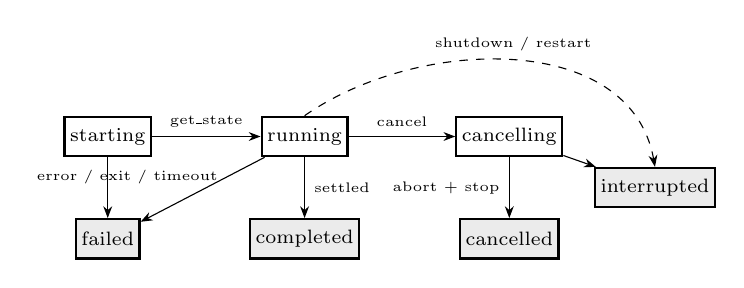
\begin{tikzpicture}[
  font=\scriptsize, >={Stealth[length=1.5mm]},
  s/.style={draw, thick, inner sep=2pt, minimum height=5mm},
  t/.style={s, fill=black!8}, l/.style={font=\tiny}]
\node[s] (st) at (0,0) {starting};
\node[s] (ru) at (2.5,0) {running};
\node[s] (ca) at (5.1,0) {cancelling};
\node[t] (co) at (2.5,-1.3) {completed};
\node[t] (fa) at (0,-1.3) {failed};
\node[t] (cc) at (5.1,-1.3) {cancelled};
\node[t] (in) at (6.95,-0.65) {interrupted};
\draw[->] (st) -- node[above, l]{get\_state} (ru);
\draw[->] (ru) -- node[above, l]{cancel} (ca);
\draw[->] (ru) -- node[right, l]{settled} (co);
\draw[->] (ru) -- node[left, l, pos=0.3]{error / exit / timeout} (fa);
\draw[->] (st) -- (fa);
\draw[->] (ca) -- node[left, l]{abort + stop} (cc);
\draw[->] (ca) -- (in);
\draw[->, dashed] (ru.north) to[out=35,in=100] node[above, l]{shutdown / restart} (in.north);
\end{tikzpicture}

\vspace{2mm}
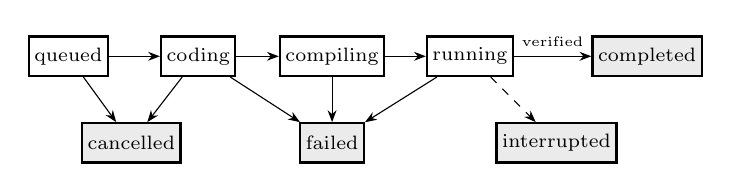
\begin{tikzpicture}[
  font=\scriptsize, >={Stealth[length=1.5mm]},
  s/.style={draw, thick, inner sep=2pt, minimum height=5mm},
  t/.style={s, fill=black!8}, l/.style={font=\tiny}]
\node[s] (q) at (0,0) {queued};
\node[s] (cd) at (1.65,0) {coding};
\node[s] (cp) at (3.35,0) {compiling};
\node[s] (rn) at (5.1,0) {running};
\node[t] (ok) at (7.35,0) {completed};
\node[t] (fl) at (3.35,-1.1) {failed};
\node[t] (cn) at (0.8,-1.1) {cancelled};
\node[t] (ir) at (6.2,-1.1) {interrupted};
\draw[->] (q) -- (cd); \draw[->] (cd) -- (cp); \draw[->] (cp) -- (rn); \draw[->] (rn) -- node[above, l]{verified} (ok);
\draw[->] (cd) -- (fl); \draw[->] (cp) -- (fl); \draw[->] (rn) -- (fl);
\draw[->] (q) -- (cn); \draw[->] (cd) -- (cn);
\draw[->, dashed] (rn) -- (ir);
\end{tikzpicture}
\caption{State machines of an agent run (top) and a Solver job (bottom).
Shaded states are terminal. Dashed edges are taken on shutdown or restart,
which interrupts any active state; a user can cancel any active job. A job
whose program is already generated passes through \emph{coding} at once.}
\label{fig:states}
\end{figure}

Runs follow the state machine at the top of Fig.~\ref{fig:states}. Creation
requires a client idempotency key. The server hashes the request; a repeated
key with the same hash returns the existing run, and a different hash is
rejected. Only one active run is allowed per conversation. The server moves
the run to \emph{running} after the agent answers \code{get\_state}, and only
then sends the prompt.

Every agent event is translated into a typed event: status, message
snapshot, text delta, reasoning delta, generation progress, tool status,
usage, or new artifact. Each is appended to an \code{events} table
\emph{before} it is broadcast. Browsers subscribe through SSE and resume from
\code{Last-Event-ID} in batches of 100 with back-pressure, so a page reload
loses nothing and does not affect the run. On the agent's \code{settled}
event, the harness fetches the persisted entries and marks the run
\emph{failed} if the last assistant message stopped with a provider error.

Finishing is a single idempotent routine. It stops the process tree, then
\emph{reconciles} the run from the agent's own append-only session file,
starting at the byte offset recorded when the run began. This recovers final
messages and chart results whose events were lost in a crash. It then closes
unfinished generations, writes explicit \emph{unknown} usage rows for model
or tool calls that ended without usage data, registers new artifacts, and
sets the terminal status. On restart, every run still marked active is
reconciled and set to \emph{interrupted}. It is never replayed, because
replaying would repeat paid model calls and side effects. Cancellation sends
the agent an \code{abort} command with a 5\,s grace period and then runs the
same finishing routine.

%======================================================================
\section{Automatic Solver Pipeline}
\label{sec:pipeline}
%======================================================================

\subsection{Batch admission}
A Solver submission names architectures, wafers (or explicit pairs), a coding
model, an idempotency key, and whether to keep automatic conclusions. All
checks run before anything is queued:
\begin{itemize}
\item pairs are de-duplicated and sorted, at most 100 per batch and 200
unfinished jobs per user;
\item a reused idempotency key must carry an identical request hash;
\item every wafer must be attached to the task. It is decoded, compared with
its registered structure and fail count, and hashed; the hash becomes the
job's \code{input\_hash};
\item an architecture whose array size differs from a paired wafer is
rejected.
\end{itemize}
One transaction then inserts the batch, one \emph{program} per architecture,
and one job per pair. Fig.~\ref{fig:seq} follows one job from submission to
its saved result.


\begin{figure*}[t]
\centering
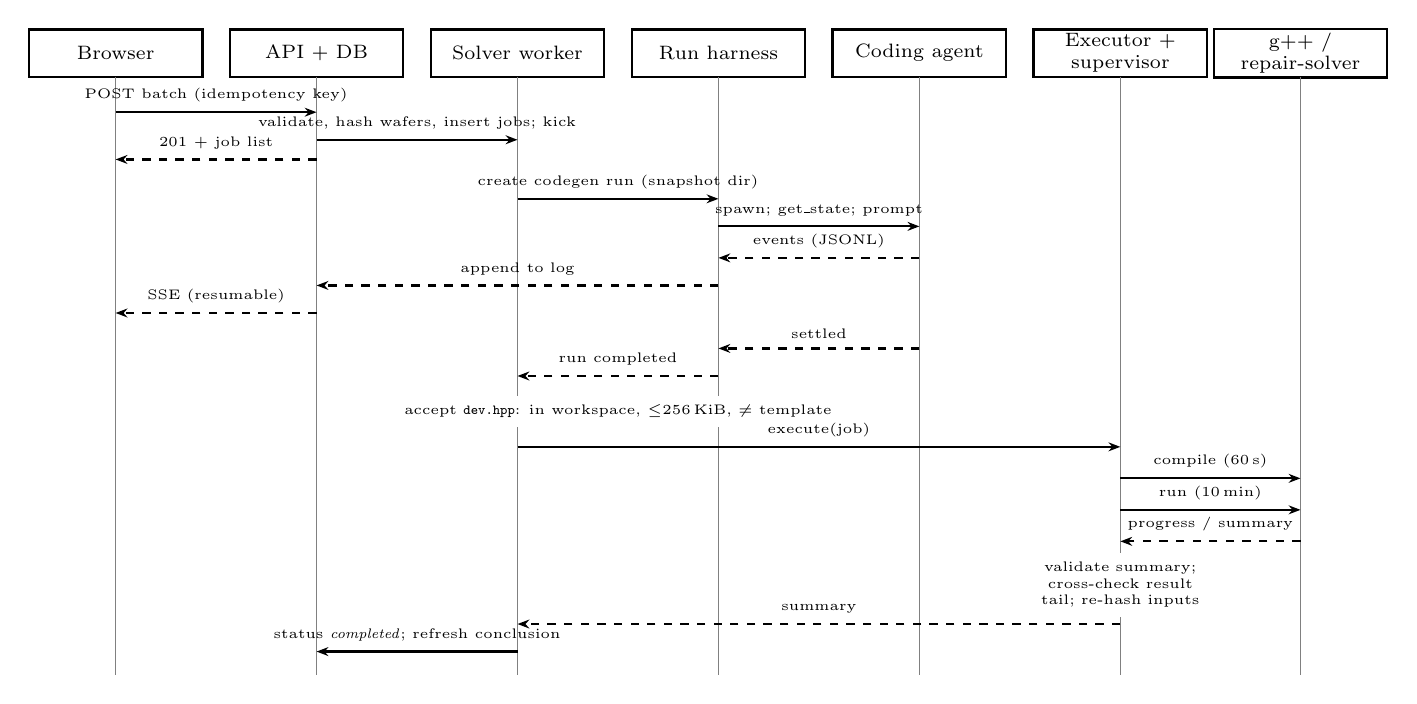
\begin{tikzpicture}[x=0.88cm, font=\scriptsize, >={Stealth[length=1.5mm]},
  hd/.style={draw, thick, align=center, minimum height=6mm, text width=21mm, inner sep=1.5pt},
  m/.style={->, thick}, r/.style={->, thick, dashed}, nt/.style={font=\tiny, align=center}]
\foreach \n/\x/\t in {u/0/Browser, a/2.9/API + DB, w/5.8/Solver worker, h/8.7/Run harness, p/11.6/Coding agent, e/14.5/Executor + supervisor, s/17.1/{g++ / repair-solver}} {
  \node[hd] (\n) at (\x,0) {\t};
  \draw[gray] (\x,-0.3) -- (\x,-7.9);
}
\draw[m] (0,-0.75) -- node[above, nt]{POST batch (idempotency key)} (2.9,-0.75);
\draw[m] (2.9,-1.1) -- node[above, nt]{validate, hash wafers, insert jobs; kick} (5.8,-1.1);
\draw[r] (2.9,-1.35) -- node[above, nt]{201 + job list} (0,-1.35);
\draw[m] (5.8,-1.85) -- node[above, nt]{create codegen run (snapshot dir)} (8.7,-1.85);
\draw[m] (8.7,-2.2) -- node[above, nt]{spawn; get\_state; prompt} (11.6,-2.2);
\draw[r] (11.6,-2.6) -- node[above, nt]{events (JSONL)} (8.7,-2.6);
\draw[r] (8.7,-2.95) -- node[above, nt]{append to log} (2.9,-2.95);
\draw[r] (2.9,-3.3) -- node[above, nt]{SSE (resumable)} (0,-3.3);
\draw[r] (11.6,-3.75) -- node[above, nt]{settled} (8.7,-3.75);
\draw[r] (8.7,-4.1) -- node[above, nt]{run completed} (5.8,-4.1);
\node[nt, fill=white] at (7.25,-4.55) {accept \texttt{dev.hpp}: in workspace, $\le$256\,KiB, $\ne$ template};
\draw[m] (5.8,-5.0) -- node[above, nt]{execute(job)} (14.5,-5.0);
\draw[m] (14.5,-5.4) -- node[above, nt]{compile (60\,s)} (17.1,-5.4);
\draw[m] (14.5,-5.8) -- node[above, nt]{run (10\,min)} (17.1,-5.8);
\draw[r] (17.1,-6.2) -- node[above, nt]{progress / summary} (14.5,-6.2);
\node[nt, fill=white, text width=30mm] at (14.5,-6.75) {validate summary; cross-check result tail; re-hash inputs};
\draw[r] (14.5,-7.25) -- node[above, nt]{summary} (5.8,-7.25);
\draw[m] (5.8,-7.6) -- node[above, nt]{status \emph{completed}; refresh conclusion} (2.9,-7.6);
\end{tikzpicture}
\caption{Sequence of one Solver job whose architecture has not been generated yet. Later jobs of the same
architecture skip the coding part and start at \emph{execute}. Solid arrows are calls, dashed arrows are responses
or streamed events.}
\label{fig:seq}
\end{figure*}

\subsection{Durable single-worker queue}
Jobs live in SQLite. A single in-process worker drains them in creation
order, which bounds compiler and solver load on the host. A submission wakes
the worker, which runs until the queue is empty. For each job, the
worker checks that the user is still enabled and the task still exists, then
obtains the program's generated code:
\begin{itemize}
\item if the program is \emph{ready}, the job reuses its stored
\code{dev.hpp}, so an architecture is generated once and evaluated on every
selected wafer;
\item if the program has \emph{failed}, its sibling jobs fail with the same
reason, which avoids paying again for a known failure;
\item otherwise the job starts a code-generation run (next subsection) and
waits on the run's event stream, with its own deadline of the run limit plus
5\,s.
\end{itemize}
A cancelled code-generation run returns the program to \emph{queued}, so a
remaining sibling job can start a fresh one.

\subsection{The code-generation contract}
\label{sec:contract}
The worker creates a dedicated conversation, ``C++ architecture coding'', in
the user's task, so the agent's work stays visible and auditable. It writes a
\code{repair-codegen/} directory containing \code{model.hpp},
\code{README.md}, a template \code{dev.hpp}, and \code{architecture.json}, an
immutable snapshot of the architecture and the paired wafer layouts. The run
uses the same harness as a chat with three differences: ambient skills are
off, the task tool is disabled, and the system prompt says to edit only
\code{dev.hpp}, not to compile or run anything, and to treat snapshot strings
as data.

The agent must implement \code{validate\_layout} and \code{build\_model}.
The model it builds contains only \code{pools} with capacities,
\code{actions} with sorted covered-fail indexes and positive pool costs, and
\code{unsupported\_constraints}. The fixed core understands exactly the
additive constraints of~\eqref{eq:model}. Any rule that does not fit must be
listed in \code{unsupported\_constraints}, and the solver then refuses the
model. A visible failure is preferred to a weakened architecture that
inflates yield. After the run, the worker accepts \code{dev.hpp} only if it
is a regular file within the workspace, at most 256\,KiB, non-empty, and
different from the template.

\subsection{Execution and acceptance}
Each job runs in \code{repair-jobs/<id>/}. The executor checks that the
wafer still matches \code{input\_hash} and its registered metadata, and copies
the wafer, \code{dev.hpp} and the three core sources into the job directory
in create-exclusive mode. It streams a text input file, hashing it as it
goes, and writes a manifest with all hashes before compiling. Each child
process is started through \code{repair-supervisor}, a process-group leader
that kills its group if the API disappears. Children get a minimal
environment (\code{PATH}, \code{LANG=C}, \code{TMPDIR}). On Linux,
\code{prlimit} caps address space (2\,GiB), CPU time and file size.
\begin{enumerate}
\item \textbf{Compile} with \code{g++ -std=c++17 -O2 -Wall -Wextra
-pedantic}, a 60\,s deadline, and a 2\,MiB log quota.
\item \textbf{Run} with a 10\,min deadline and an 8\,MiB log quota. Stdout
must be JSONL with lines under 1\,MiB, containing only \code{progress}
events and exactly one \code{summary}. Progress must be monotone and refer
to the full region count; it is written to the job at most every 200\,ms.
\item \textbf{Validate the summary} against invariants computed
independently from the decoded wafer: totals equal the wafer layout;
fail-free regions and chips match the decoder's counts; passed $=$
fail-free $+$ repaired; passed $+$ unresolved $=$ total; and both yields
equal their ratios within $10^{-12}$.
\item \textbf{Cross-check} that the last line of \code{result.jsonl} is a
summary identical to the one on stdout.
\item \textbf{Re-hash} the source wafer, its copy, \code{dev.hpp}, the
input text and every core source, and reject the job if anything changed
during execution.
\end{enumerate}
Only then is the job marked \emph{completed}, and the manifest receives the
summary and completion time. On any failure the manifest records the time and
the error. Table~\ref{tab:failures} lists how the harness handles common
failures. Inside the solver, each region's selected actions are re-checked
against coverage and capacities independently of the search bookkeeping,
so every \emph{repaired} region has a verified witness.

\begin{table}[t]
\centering
\caption{Failure modes and harness responses}
\label{tab:failures}
\setlength{\tabcolsep}{3pt}
\renewcommand{\arraystretch}{1.05}
\begin{tabular}{p{30mm}p{52mm}}
\toprule
Failure & Response \\
\midrule
Agent hangs or loops & run deadline; group kill incl.\ detached tool groups \\
Agent leaves template / oversized code & program \emph{failed}; siblings fail fast, no re-billing \\
Unsupported architecture rule & model rejected with the declared reason \\
Code does not compile & job \emph{failed}; \code{compile.log} downloadable \\
Solver floods output & log quota exceeded $\rightarrow$ group killed \\
Malformed or inconsistent summary & job \emph{failed}; no yield shown \\
Input or code modified during run & hash mismatch $\rightarrow$ job \emph{failed} \\
User cancels & abort, kill, \emph{cancelled}; program re-queued \\
API process dies & IPC closes $\rightarrow$ supervisors kill their trees \\
Service restart & active runs/jobs \emph{interrupted}; never replayed \\
\bottomrule
\end{tabular}
\end{table}

\subsection{Two further harnesses}
The same pattern (agent writes, harness validates and archives) automates
two other workflows. \textbf{Architecture previews:} the agent writes a
browser-executed \code{draw.mjs}, a scene file and its generating script,
then runs a publisher that accepts only small regular files in the run
directory, checks the scene against the task's architecture fingerprint,
and archives a hashed manifest (\code{pixel-architecture-preview/v1})
without overwriting earlier versions; the browser runs \code{draw} with an
injected Pixi~\cite{pixi} context. \textbf{Exact evaluation:} for HiGHS,
\code{plan} fingerprints data and sources without solving, and \code{run}
accepts only a plan, snapshots every source and checks that none changed.

\subsection{Automatic conclusions}
After every terminal job, the worker refreshes the task's saved conclusion
(if enabled for the batch): a database snapshot of every job's architecture
fingerprint, input hash, engine and summary, rewritten only when it
changes. Conclusions thus need no chat artifacts or open browser; they
compare only shared wafer inputs and show missing results as gaps.

%======================================================================
\section{Solver Core}
\label{sec:solver}
%======================================================================

The default engine, \emph{repairMost}, is a capacity-aware greedy
max-coverage heuristic, the classical set-cover rule~\cite{johnson1974}
with budget checks. It uses an inverted fail$\rightarrow$action index and a
lazy max-heap with per-action generation counters, so stale entries are
skipped and the run time is near-linear in the number of incidences. An
action that no longer fits is dropped permanently, which is safe because
capacity only shrinks. Ties are broken by the smallest action id, which
keeps runs deterministic. The model is validated first (unique in-range
coordinates, unique bounded ids, strictly increasing indexes, and global
bounds of $10^6$ actions and $1.6\times10^7$ incidences), and the result is
re-checked afterwards. For exact answers, a Python framework solves the same
model as a binary program with HiGHS~\cite{huangfu2018} (single thread,
fixed seed, zero gap, per-region time limit). It labels each region
\emph{repairable}, \emph{unrepairable} or \emph{unknown}, and reports a yield
interval whenever any region is unknown.

%======================================================================
\section{The System in Operation}
\label{sec:operation}
%======================================================================

\begin{figure*}[t]
\centering
\begin{tabular}{@{}c@{\hspace{2mm}}c@{}}
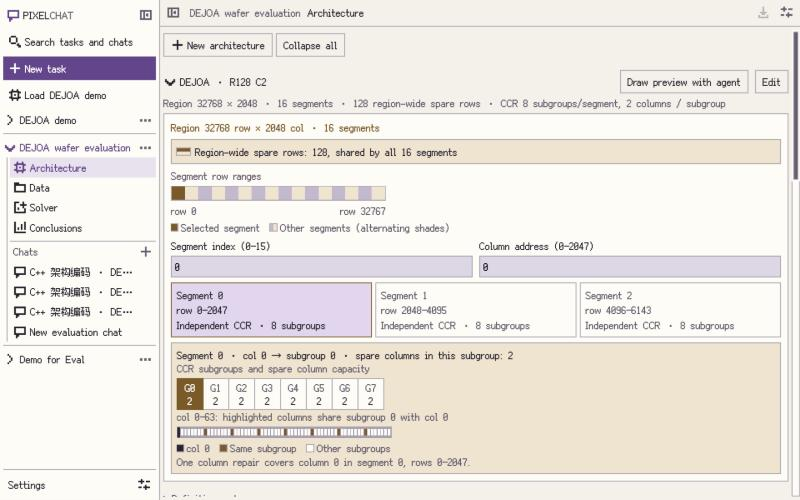
\includegraphics[width=0.49\textwidth]{figures/ui-architecture.jpg} &
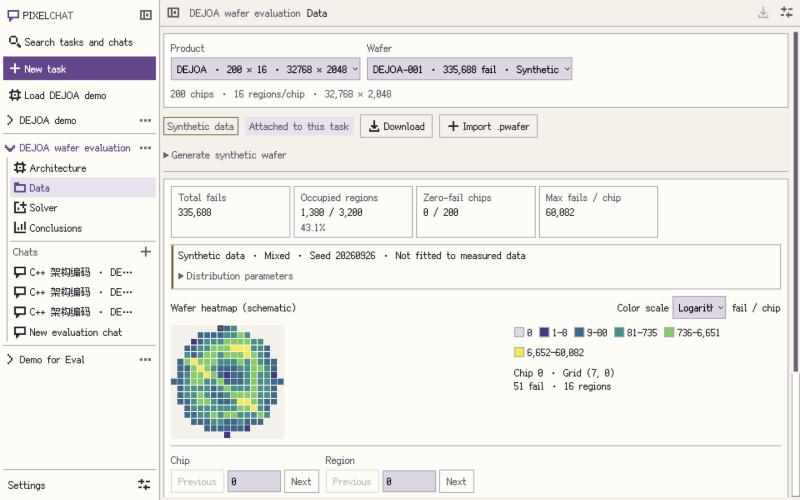
\includegraphics[width=0.49\textwidth]{figures/ui-data.jpg} \\
\scriptsize (a) Architecture: 16 segments, region-wide rows, 8 CCR subgroups &
\scriptsize (b) Data: wafer DEJOA-001, 335\,688 fails, log-scale heatmap \\[1mm]
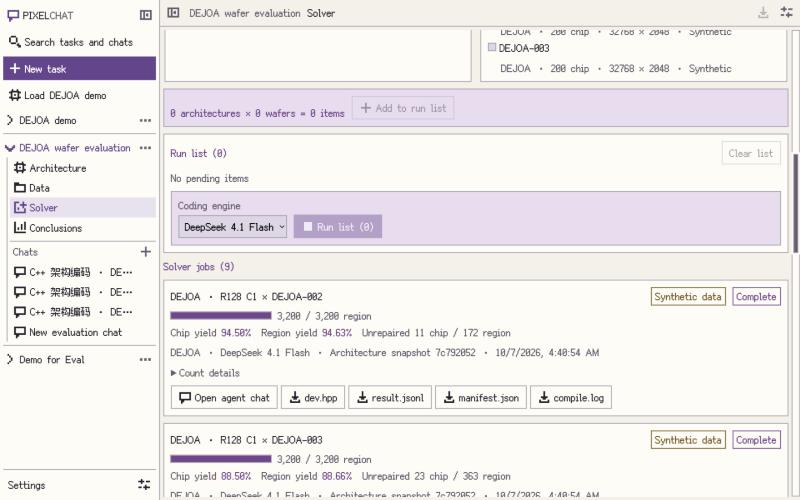
\includegraphics[width=0.49\textwidth]{figures/ui-solver-jobs.jpg} &
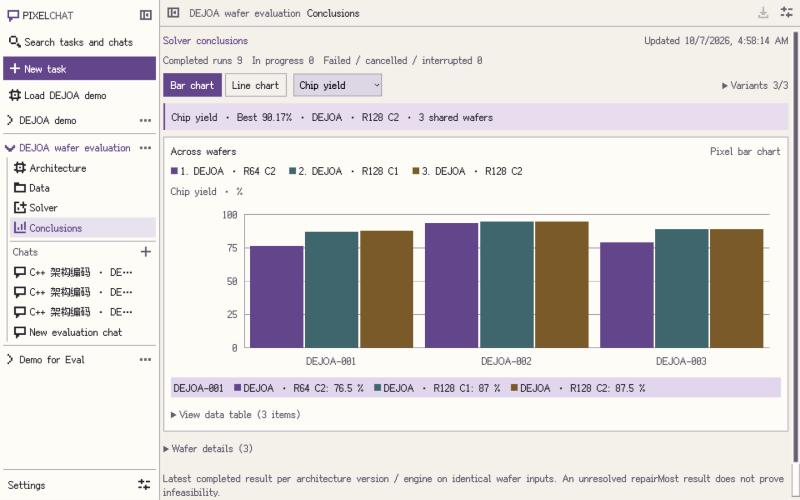
\includegraphics[width=0.49\textwidth]{figures/ui-conclusions.jpg} \\
\scriptsize (c) Solver: completed jobs with progress, yields and artifacts &
\scriptsize (d) Conclusions: saved automatically, compared on shared wafers \\
\end{tabular}
\caption{The DEJOA task in the running system (English UI, 1440$\times$900
viewport). The user defines architectures (a) and attaches wafers (b), then
submits one batch. The harness generates, compiles, runs and verifies each
job (c) and saves conclusions as jobs finish (d). Every job card links to
its coding chat and to \code{dev.hpp}, \code{result.jsonl},
\code{manifest.json} and \code{compile.log}.}
\label{fig:ui}
\end{figure*}

\subsection{Setup}
We loaded the built-in DEJOA demo. It contains three synthetic wafers
(DEJOA-001 to 003; 200 chips $\times$ 16 regions; \emph{mixed} spatial
pattern; seeds 20260926--28; mean 1600 fails per chip) and three
architectures with 16 segments of 2048 rows and $G=8$: \textbf{R64\,C2}
(64 spare rows, 2 per subgroup), \textbf{R128\,C1} and \textbf{R128\,C2}. One
submission queued all nine pairs with \code{deepseek-flash} as the coding
model. Fig.~\ref{fig:ui} shows the four task views during this study.

\subsection{Timeline}

\begin{figure}[t]
\centering
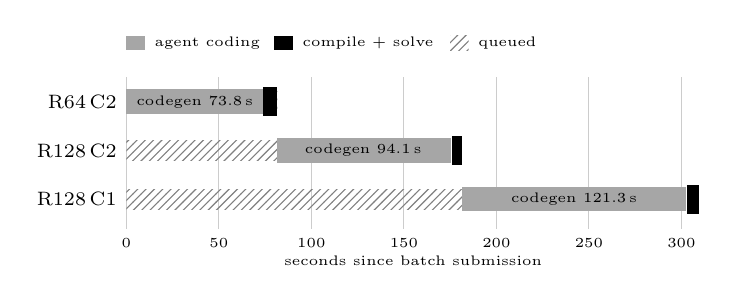
\begin{tikzpicture}[x=0.0235cm, y=0.62cm, font=\scriptsize]
\foreach \x in {0,50,100,150,200,250,300} {
  \draw[gray!40] (\x,0.4) -- (\x,3.5);
  \node[below, font=\tiny] at (\x,0.4) {\x};
}
\node[font=\tiny] at (155,-0.25) {seconds since batch submission};
% lane labels
\node[left] at (0,3) {R64\,C2};
\node[left] at (0,2) {R128\,C2};
\node[left] at (0,1) {R128\,C1};
% queued waits
\fill[pattern=north east lines, pattern color=gray] (0,2.8) rectangle (81.64,3.2);
\fill[pattern=north east lines, pattern color=gray] (0,1.8) rectangle (81.64,2.2);
\fill[pattern=north east lines, pattern color=gray] (0,0.8) rectangle (181.44,1.2);
% codegen runs
\fill[black!35] (0.02,2.75) rectangle (73.83,3.25);
\fill[black!35] (81.64,1.75) rectangle (175.73,2.25);
\fill[black!35] (181.44,0.75) rectangle (302.70,1.25);
% exec: compile+solve for 001,003,002
\fill[black] (73.91,2.7) rectangle (78.93,3.3);
\fill[black] (78.99,2.7) rectangle (80.29,3.3);
\fill[black] (80.34,2.7) rectangle (81.63,3.3);
\fill[black] (175.81,1.7) rectangle (178.76,2.3);
\fill[black] (178.83,1.7) rectangle (180.06,2.3);
\fill[black] (180.11,1.7) rectangle (181.44,2.3);
\fill[black] (302.90,0.7) rectangle (306.42,1.3);
\fill[black] (306.49,0.7) rectangle (307.98,1.3);
\fill[black] (308.02,0.7) rectangle (309.41,1.3);
\node[font=\tiny] at (37,3.0) {codegen 73.8\,s};
\node[font=\tiny] at (128,2.0) {codegen 94.1\,s};
\node[font=\tiny] at (242,1.0) {codegen 121.3\,s};
% legend
\fill[black!35] (0,4.05) rectangle (10,4.35); \node[right, font=\tiny] at (10,4.2) {agent coding};
\fill[black] (80,4.05) rectangle (90,4.35); \node[right, font=\tiny] at (90,4.2) {compile + solve};
\fill[pattern=north east lines, pattern color=gray] (175,4.05) rectangle (185,4.35); \node[right, font=\tiny] at (185,4.2) {queued};
\end{tikzpicture}
\caption{Timeline of the nine-job batch, from job and run timestamps in the
database and job manifests. The single worker processes one architecture at
a time; after one coding run, its three wafers are compiled and solved in
1.2--5.0\,s each.}
\label{fig:timeline}
\end{figure}

Fig.~\ref{fig:timeline} shows the batch as recorded by the harness. It
finished in 309.4\,s. The three code-generation runs took 73.8, 94.1 and
121.3\,s, together 289\,s or 93.5\,\% of the wall time. The nine
compile-and-solve phases, measured from manifest creation to completion,
took 1.23--5.02\,s each and 19.5\,s in total. The gap between a coding run
ending and its first compile was under 0.2\,s. Because programs are shared,
each coding run serves three jobs. Without sharing, the batch would have
needed nine coding runs, roughly tripling the coding time. The worker is
single-threaded by design, so the second and third architectures waited 82
and 181\,s in the queue. Coding runs spend most of their time waiting on the model provider rather
than on local CPU, so running them concurrently while keeping compilation
and solving serialized is the most direct way to shorten such batches.

\subsection{What the agent did}

\begin{table}[t]
\centering
\caption{Code-generation runs recorded by the harness}
\label{tab:codegen}
\setlength{\tabcolsep}{3pt}
\begin{tabular}{lrrr}
\toprule
 & R64\,C2 & R128\,C2 & R128\,C1 \\
\midrule
Wall time (s) & 73.8 & 94.1 & 121.3 \\
Model calls & 8 & 10 & 15 \\
Tools: read/bash/write & 7/4/2 & 11/6/1 & 11/9/2 \\
Tokens in/out (k) & 21.3/15.0 & 27.9/20.3 & 37.3/21.9 \\
Cache-read (k) & 148 & 254 & 408 \\
Events & 14\,889 & 20\,067 & 21\,680 \\
\code{dev.hpp} lines/B & 280/11\,983 & 280/12\,433 & 212/9\,799 \\
\bottomrule
\end{tabular}
\end{table}

\begin{figure}[t]
\centering
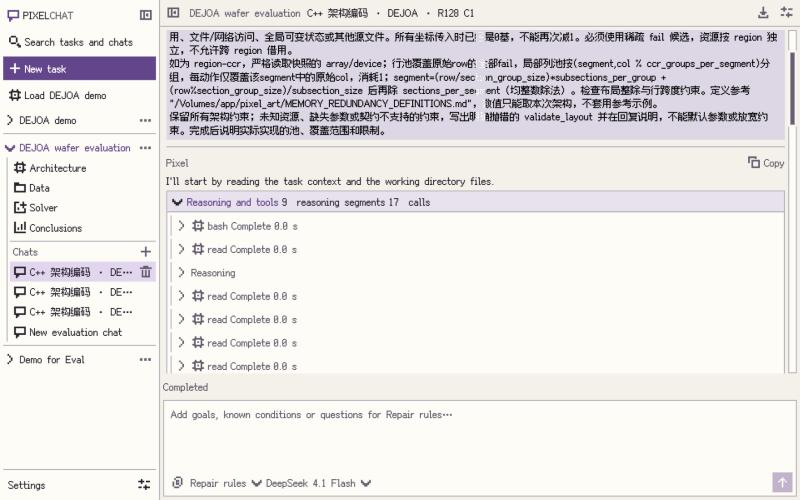
\includegraphics[width=\columnwidth]{figures/ui-codegen-trace.jpg}
\caption{A code-generation chat created by the harness. The top shows the
generated instruction (written in Chinese by the harness) with the
workspace path, the edit-only rule and the segment formula; below, the
agent's tool calls (\code{bash}, \code{read}) are listed as they were
streamed and persisted.}
\label{fig:trace}
\end{figure}

Table~\ref{tab:codegen} summarizes the three coding runs, and
Fig.~\ref{fig:trace} shows one of them as the user sees it. All three
completed, and their code compiled without warnings (empty
\code{compile.log}). Most events are streaming deltas: 63--74\,\% are
reasoning deltas. Persisting them lets the page show the agent's progress
live and replay it after a reload. Usage was recorded per call; since no
verified price was configured for this model, cost is reported as unknown
rather than estimated.

The tool traces also exposed a limit of instruction-only scoping. The prompt
confines edits to \code{dev.hpp}, and the acceptance checks confirm that
only \code{dev.hpp} was taken from the agent. However, the agents' shell
commands also \emph{read} outside the workspace: they listed the solver
sources, and one run searched the harness's own \code{runner.ts} for the
compiler flags. Reading was harmless here and even useful, since it matched
the agent's code to the real compile command. Still, it shows that the
current harness controls what is \emph{accepted}, not what is
\emph{observed}. Section~\ref{sec:lessons} returns to this point.

\subsection{Engineering effort and development capacity}
\label{sec:effort}

The harness's practical benefit is to move architecture-specific coding,
compilation, repeated wafer runs and result bookkeeping off the engineer's
critical path. We quantify the potential labor saving with a transparent
planning scenario, separate from the measured machine timeline. Assume a
manual implementation rate of 100 lines per eight-hour engineer-day, and
budget at most two engineer-hours per harness-assisted configuration for
setup, supervision, architectural model review and result review. The
two-hour ceiling is an assumption for this calculation, not an observed
upper bound across arbitrary architectures.

For $N$ independently implemented configurations with generated file lengths
$L_i$, the baseline and assisted-effort budget are
\begin{equation}
H_{\mathrm{manual}}=\frac{8}{100}\sum_{i=1}^{N}L_i,
\qquad H_{\mathrm{budget}}=2N.
\label{eq:effort}
\end{equation}
The recorded files have 280, 280 and 212 lines (Table~\ref{tab:codegen}).
We charge the two-hour allowance once per configuration, rather than once
per wafer, because one generated program serves all three wafers.
Table~\ref{tab:effort} gives the resulting estimates.

\begin{table}[t]
\centering
\caption{Estimated engineer-hours under the stated planning assumptions}
\label{tab:effort}
\setlength{\tabcolsep}{3pt}
\begin{tabular}{lrrrr}
\toprule
Configuration & Lines & Manual & Budget & Released \\
\midrule
R64\,C2 & 280 & 22.40 & 2.00 & 20.40 \\
R128\,C2 & 280 & 22.40 & 2.00 & 20.40 \\
R128\,C1 & 212 & 16.96 & 2.00 & 14.96 \\
\midrule
Total & 772 & 61.76 & 6.00 & 55.76 \\
\bottomrule
\end{tabular}
\end{table}

For this three-configuration batch, the manual baseline is 7.72
engineer-days, while the assisted budget is 0.75 engineer-day. Thus 55.76
hours, or 6.97 engineer-days, can be reassigned to additional architecture
candidates, fail-pattern coverage, model validation or design refinement.
The estimated effort reduction is
$1-6/61.76=90.3\,\%$. At equal staffing and the same configuration mix,
the capacity multiplier is $61.76/6=10.3$: one engineer-week of 40 hours
supports about 1.9 configurations under the manual baseline versus 20 under
the assisted budget. This is a potential acceleration of configuration
evaluation, not a measured 10.3$\times$ speedup of the entire development
cycle. At a fully loaded hourly labor rate $w$, the estimated released labor
cost is $55.76w$; no salary or monetary saving is assumed here.

These estimates use gross file line counts, including comments and blank
lines, as a proxy for implementation size. They assume manual implementations
are written independently; reuse of an existing model or a parameterized
template would reduce the manual baseline and the estimated saving.
Neither manual productivity nor actual engineer attention was measured in
this study. Complex modeling or review may exceed the two-hour allowance.
The measured 309.4-second batch demonstrates automated execution time;
it does not substitute for a human-effort measurement or semantic review.

\subsection{Results and audit}

\begin{table}[t]
\centering
\caption{Region / chip yield (\%): greedy engine vs.\ column-first witnesses (both lower bounds)}
\label{tab:results}
\setlength{\tabcolsep}{3pt}
\begin{tabular}{llrrr}
\toprule
Wafer & Method & R64\,C2 & R128\,C1 & R128\,C2 \\
\midrule
\multirow{2}{*}{001} & greedy & 81.5 / 76.5 & 87.5 / 87.0 & 88.2 / 87.5 \\
 & col.-first & 92.3 / 92.0 & 92.0 / 92.0 & 94.5 / 94.5 \\
\multirow{2}{*}{002} & greedy & 93.2 / 93.0 & 94.6 / 94.5 & 95.1 / 94.5 \\
 & col.-first & 96.2 / 96.0 & 96.0 / 96.0 & 96.5 / 96.5 \\
\multirow{2}{*}{003} & greedy & 81.9 / 78.5 & 88.7 / 88.5 & 89.2 / 88.5 \\
 & col.-first & 92.0 / 92.0 & 92.0 / 92.0 & 93.5 / 93.5 \\
\midrule
\multirow{2}{*}{Pooled} & greedy & 85.5 / 82.7 & 90.3 / 90.0 & 90.8 / 90.2 \\
 & col.-first & 93.5 / 93.3 & 93.3 / 93.3 & 94.8 / 94.8 \\
\bottomrule
\end{tabular}
\end{table}

All nine jobs passed every acceptance check. Their greedy yields are the
``greedy'' rows of Table~\ref{tab:results}, and they appear unchanged in
Fig.~\ref{fig:ui}(c,d). Only 1 of 600 chips was fail-free before repair, so
chip yield gain is within 0.2 points of chip yield. Taken at face value, the
greedy results favor spare rows: R128\,C1, with 256 spares per region,
beats R64\,C2, with 320, on every wafer.

Because the harness records unrepaired regions as \emph{unresolved} rather
than infeasible, and keeps per-region records, these results could be
audited. Defective regions hold 217--413 fails on average across 32768 rows,
so nearly every action covers exactly one fail and all gains tie. Ties go to
the smallest id. The generated ids begin with \code{row} for rows and
\code{seg} or \code{segment} for columns, so greedy spends row spares first:
rows are 52--81\,\% of its selected actions. We therefore applied a
\emph{column-first} construction offline. In each CCR pool it takes the $C$
columns with the most fails, covers the remaining fails with rows, and
accepts the region if at most $R$ distinct rows are needed. Each accepted
region has an explicit witness satisfying~\eqref{eq:model}. It repaired every
region greedy repaired, plus 44--343 more per job. It raised pooled region
yield by 7.9, 3.1 and 4.0 percentage points, computed from unrounded counts,
and reversed the R64\,C2 vs.\ R128\,C1
ranking. The regions that remain unrepaired form whole high-fail chips; for
example, on wafers 001 and 003 under R128\,C1, region and chip yield are both
exactly 92.0\,\%, so the failed regions are 16 complete chips. The fix
belongs in the solver: tie-breaking should account for pool scarcity. The
point for the harness is that a heuristic failure was never reported as
infeasibility, and that every input needed to check the numbers was
preserved.

%======================================================================
\section{Lessons and Limitations}
\label{sec:lessons}
%======================================================================

\textbf{Narrow what is accepted.} Restricting the agent to two model-entry
functions behind a validating core, with an explicit list of unsupported
constraints, lets the harness reject compilation failures, malformed models
and invalid repair witnesses, so batches run unattended. It is not a
correctness check: whether the model matches the architecture remains an
engineering review.

\textbf{Make the log the source of truth.} Persisting every event before
broadcasting it, and reconciling from the agent's own session file, made
reloads, crashes and cancellations uneventful. Marking interrupted work
instead of replaying it avoided duplicate model charges.

\textbf{Share expensive steps.} Code generation dominated wall time (93.5\,\%).
Sharing one program per architecture across wafers is the largest saving;
concurrent coding runs would be the next.

\textbf{Reinvest released engineering effort.} Under the assumptions of
Section~\ref{sec:effort}, the harness cuts estimated implementation and
evaluation effort by 90.3\,\%, releasing almost seven engineer-days in the
three-configuration study. The useful development effect is broader design
exploration and more time for semantic review, rather than removing the
engineer from the decision process.

\textbf{Scope reads, not just writes.} The agent read files outside its
workspace. A future version should run agent tools in an OS-level sandbox
(a container or a restricted user with a read-only view of the needed files)
instead of relying on instructions. Process limits today contain mistakes;
they do not isolate a malicious agent.

\textbf{Other limitations.} The run limits apply per process. The worker is
single-threaded. All evaluation data are synthetic and use 200-chip wafers.
Greedy and column-first yields are lower bounds, and HiGHS has not yet been
run on these inputs. Testing is manual.

%======================================================================
\section{Conclusion}
%======================================================================

The harness lets a user go from a list of architectures and wafers to saved,
comparable conclusions with one submission, while the agent writes the
architecture-specific code. Its central choices are supervised process trees
with explicit deadlines, a durable event log with reconciliation and
non-replaying recovery, a single queue that shares code generation across
wafers, and acceptance only after protocol, invariant and integrity checks.
A recorded nine-job batch completed in about five minutes, mostly spent
on code generation, and its preserved per-region records made it possible
to improve region yield lower bounds by up to 10.7 percentage points.
Under a 100-lines-per-engineer-day baseline and a two-hour assisted allowance
per configuration, the three configurations release an estimated 55.76
engineer-hours (90.3\,\%) and support 10.3$\times$ as many configuration
evaluations at equal staffing. These conditional savings can accelerate
architecture exploration and free engineering effort for model review;
they are separate from the measured execution time. Next steps are
OS-level sandboxing of agent tools, concurrent coding runs,
scarcity-aware tie-breaking, and exact HiGHS runs inside the same pipeline.

\section*{Acknowledgment}
The interface font is Fusion Pixel
12px~\cite{fusionpixel}, used under its open license.

\bibliographystyle{IEEEtran}
\bibliography{refs}

\end{document}
